%% NEExT Reddit Graph Classification Manuscript
%% Starting from scratch - blank template
%%
\documentclass[linenumbers]{aastex701}

%% Custom commands
\newcommand{\neext}{NEExT}

%% Set path for figures
\graphicspath{{figures/}}

%% Running header - UPDATE LATER
%%\shorttitle{}
%%\shortauthors{}

%% Dates - ADD AS WE PROGRESS
%%\received{}
%%\revised{}
%%\accepted{}

\begin{document}

\title{[Title Goes Here]}

%% Author information - TO BE ADDED
\author{Author Name}
\affiliation{Institution}
\email{email@domain.edu}

%% Abstract
\begin{abstract}

[Abstract will be written as experiments progress. 300 word limit for PASP.]

\end{abstract}

%% Keywords
\keywords{[Add keywords]}

%% ============================================================================
%% INTRODUCTION
%% ============================================================================
\section{Introduction} \label{sec:intro}

[Introduction to be written]

%% ============================================================================
%% BACKGROUND
%% ============================================================================
\section{Background} \label{sec:background}

[Background section]

%% ============================================================================
%% RELATED WORK
%% ============================================================================
\section{Related Work} \label{sec:related}

[Related work section]

%% ============================================================================
%% METHODS
%% ============================================================================
\section{Methods} \label{sec:methods}

[Methods section]

%% ============================================================================
%% EXPERIMENTS
%% ============================================================================
\section{Experiments} \label{sec:experiments}

[Experiments and results]

%% ============================================================================
%% RESULTS
%% ============================================================================
\section{Results} \label{sec:results}

\begin{figure}[ht!]
\centering
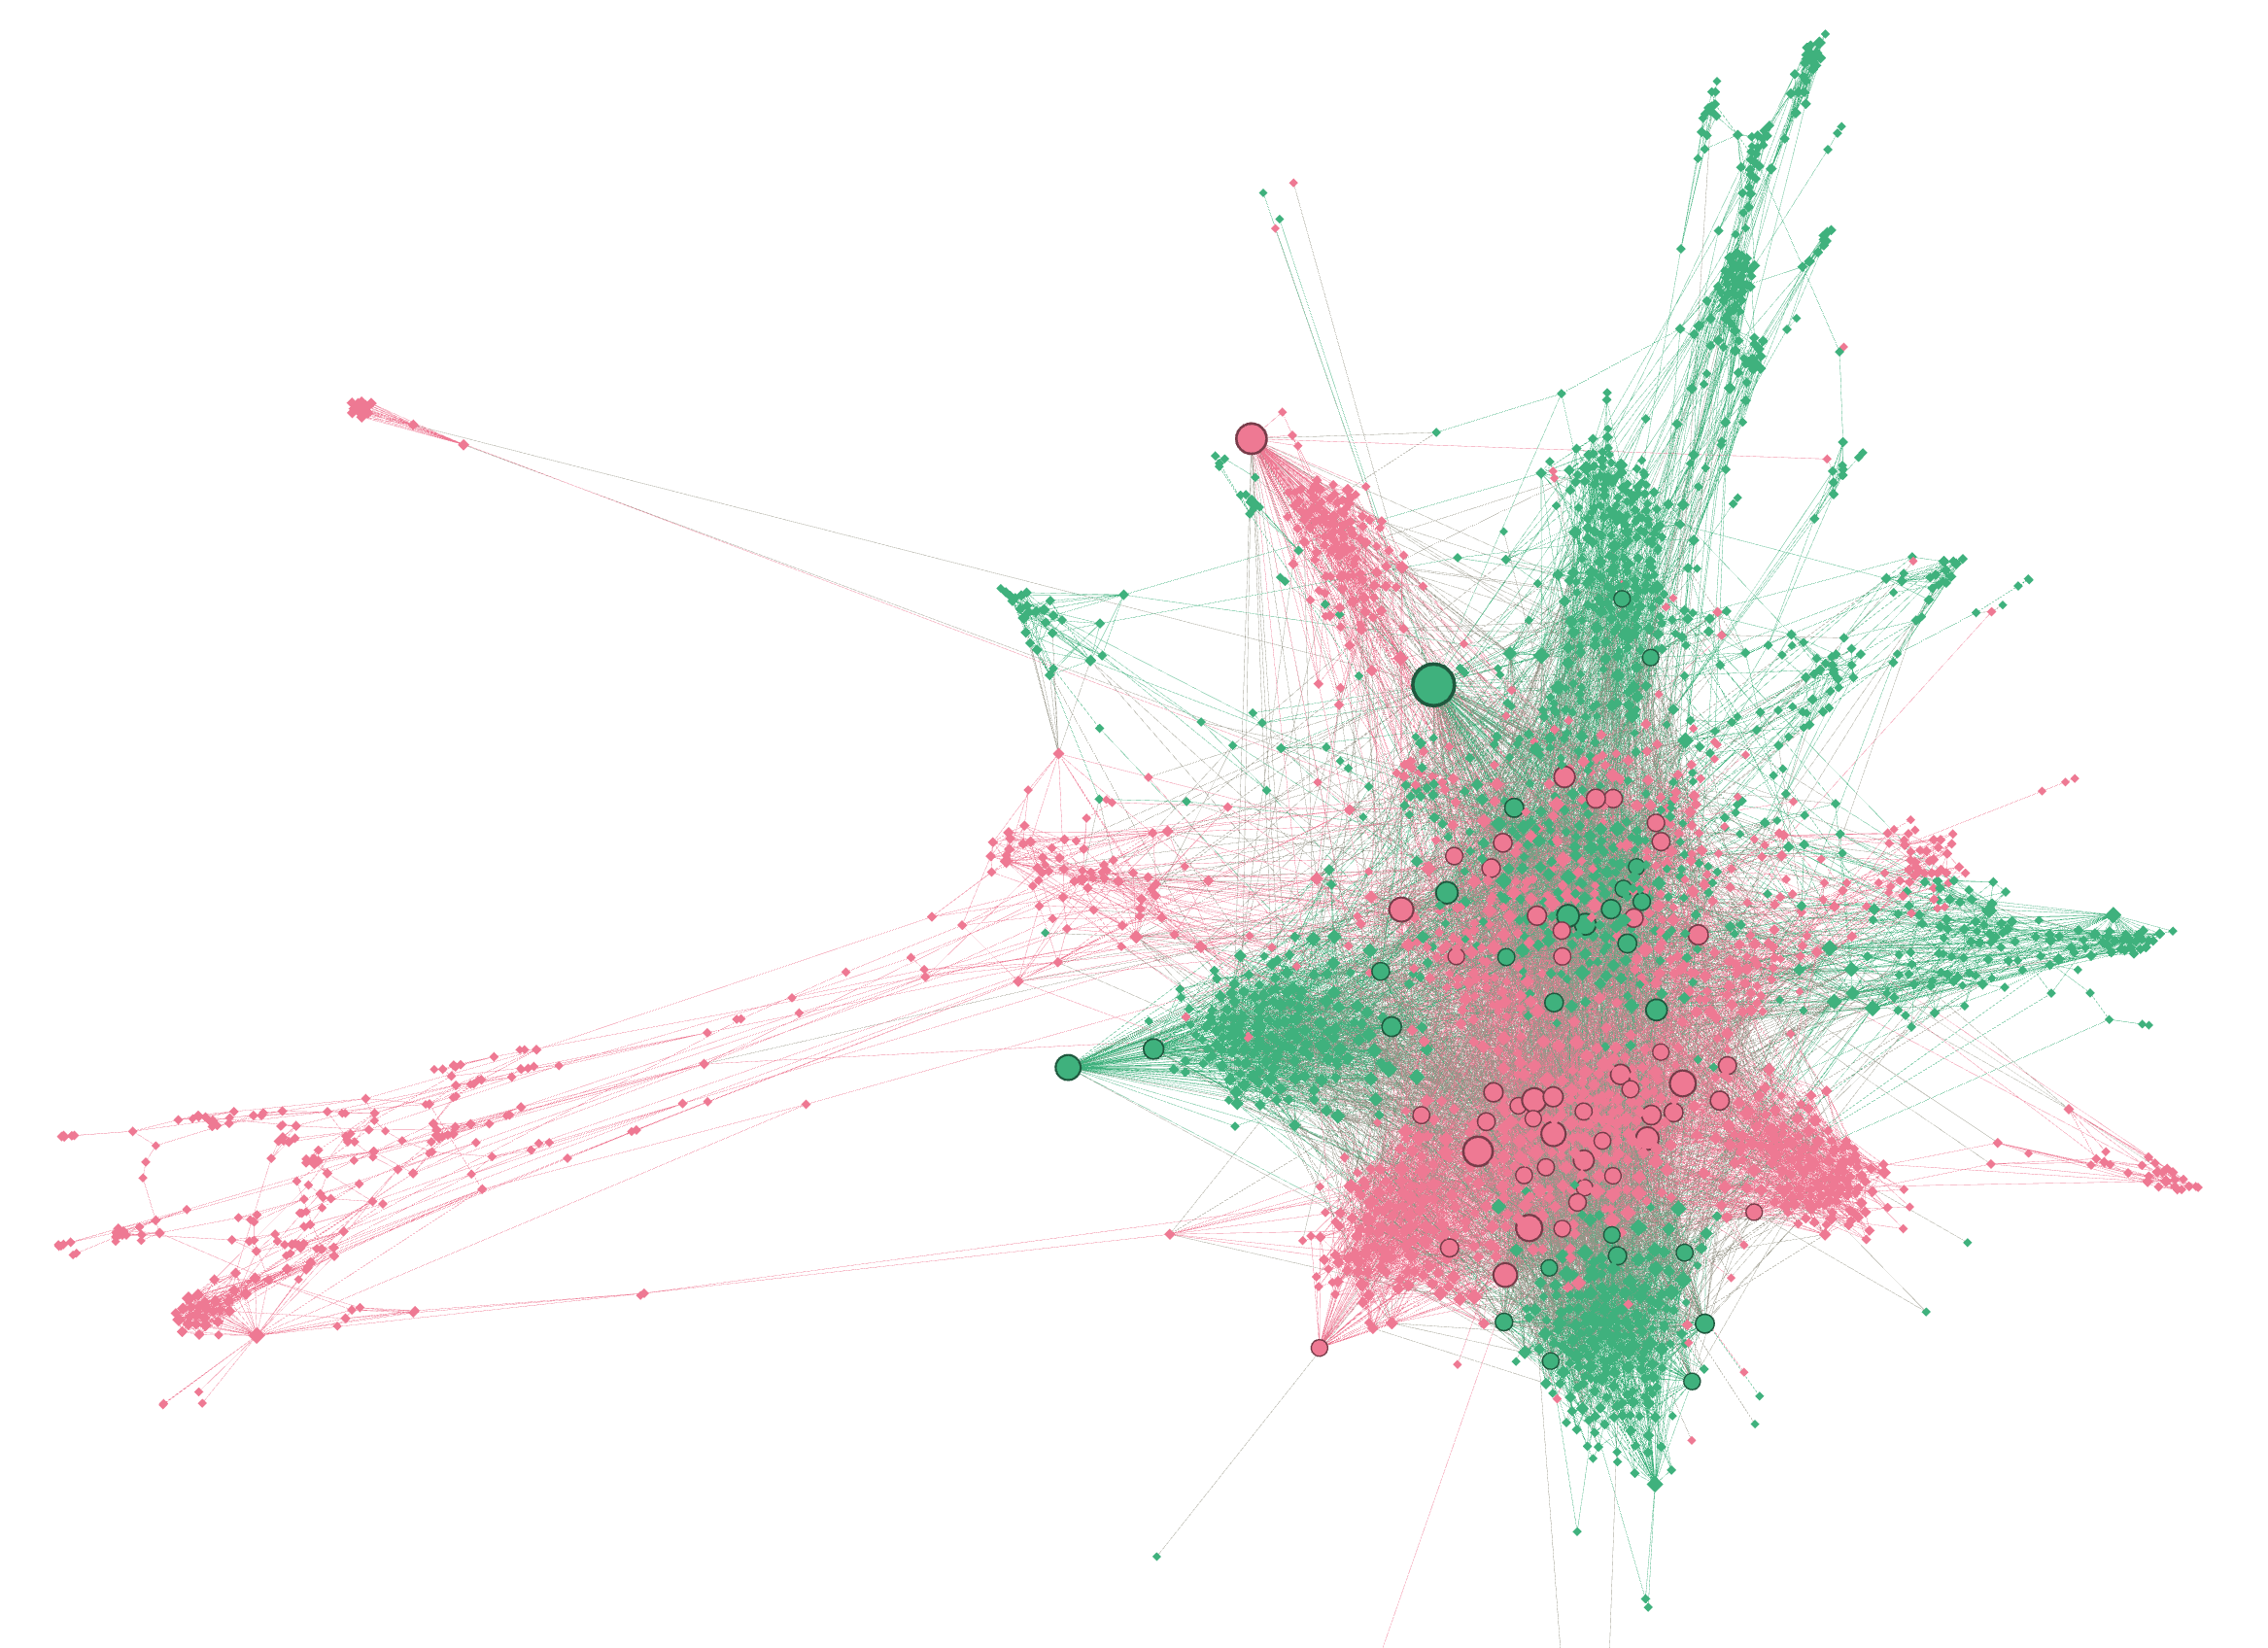
\includegraphics[width=0.85\linewidth]{reddit_2_percent_graph.png}
\caption{Visualization of the Reddit 2\% sample network (2,696 nodes, 15,885 edges). Blue nodes represent serious subreddits (news, science, technology) while red nodes represent entertainment subreddits (gaming, media, art).}
\label{fig:reddit_network}
\end{figure}

[Results section]

%% ============================================================================
%% DISCUSSION
%% ============================================================================
\section{Discussion} \label{sec:discussion}

[Discussion section]

%% ============================================================================
%% CONCLUSION
%% ============================================================================
\section{Conclusion} \label{sec:conclusion}

[Conclusion]

%% ============================================================================
%% ACKNOWLEDGMENTS
%% ============================================================================
\begin{acknowledgments}
[Acknowledgments]
\end{acknowledgments}

%% ============================================================================
%% BIBLIOGRAPHY
%% ============================================================================
\bibliography{neext_reddit}
\bibliographystyle{aasjournalv7}

\end{document}